\documentclass[12pt]{report}
\usepackage[print,nopanel]{pdfscreen}
%\begin{print}
\usepackage{lipsum}% http://ctan.org/pkg/lipsum
\usepackage{titletoc}% http://ctan.org/pkg/titletoc
%\section{type}

\usepackage{lastpage}
\usepackage{macro/macro}
\usepackage{float}
\usepackage{fancyhdr}
\usepackage{verbatim}
\usepackage[Glenn]{fncychap}
\lhead{\large\bfseries DRB}
\usepackage[left=2.5cm, right=1.5cm, top=2.5cm, bottom=1.5cm]{geometry}
\pagestyle{fancy}
%\end{print}
\margins{2.5cm}{1.5cm}{1.5cm}{1.5cm}
\begin{screen}

\renewcommand{\encodingdefault}{T1}
\usepackage{setspace}
\linespread{1.5}
\renewcommand{\rmdefault}{ptm}
\end{screen}
\screensize{8cm}{9cm}
\overlay{overlay8.pdf}
\usepackage{graphicx}

\begin{document}
\newcommand{\centertext}[1]{\begin{center}\textbf{#1}\end{center}}
\newcommand{\student}{\vskip 2.5cm}
\newcommand{\supervisor}{\vskip 2cm}
\newcommand{\stamp}{\vskip 2.5cm}
\newcommand{\HRule}{\rule{\linewidth}{0.5mm}}
\newcommand{\projecttitle}{\Huge \bf{Design Reinforcement of Beam \\ (DRB)}\vskip 0.1in}
\newcommand{\tab}[1]{\hspace{.4\textwidth}\rlap{#1}}
\newcommand{\itab}[1]{\hspace{.05\textwidth}\rlap{#1}}
\newcommand{\logo}[1]{\includegraphics[scale=0.16]{#1}}
\newcommand{\submitted}{
\vskip 0.4in
\textnormal{Submitted for partial fulfilment of the Degree\\
of\\
Bachelor of Technology\\
(Computer Science and Engineering)\\
}
\vskip 2.5cm
%\image{0.7}{images/gne.png}{}
\logo{images/gne.png}
\vskip 3.0cm
\begin{minipage}{0.4\textwidth}
\begin{flushleft} \large
{Submitted By:}\\
\textnormal{Tamandeep Singh\\
1410939} % Your name
\end{flushleft}
\end{minipage}
~
\begin{minipage}{0.4\textwidth}
\begin{flushright} \large
{Submitted To:} \\
\textnormal{Kapil Sharma\\ Training Coordinator\\ CSE Department \\                                                                                     } % Supervisor's Name
\end{flushright}
\end{minipage}\\[2cm]
\HRule \\[0.4cm]

\textnormal{Department of Computer Science \& Engineering \\
Guru Nanak Dev Engineering College \\
Ludhiana 141006}
}


\newcommand{\pagetitle}{\begin{center}
\projecttitle
\Large\textbf{}\\
\submitted
\vskip 1cm

\end{center}}
\newcommand{\openoffice}{\textbf{OpenOffice}}
\newcommand{\frontmatter}[1]{\begin{Large} \textbf{#1} \end{Large}}
\newcommand{\ppttitle}{\begin{center}
\end{center}}


\begin{screen}
\ppttitle
\end{screen}
\footskip 0.7cm
\thispagestyle{empty} 
\pagetitle
\newpage
\pagenumbering{Roman}
\cfoot{\thepage}

\begin{Large}
\centertext{Acknowledgement}
\end{Large}

I, student of Guru Nanak Dev Engineering College, Ludhiana, have taken efforts in this project.
However, it would not have been possible without the kind support and help of many individuals
and organizations. I would like to extend my sincere thanks to all of them.\\

The author is highly grateful to Dr. M.S. Saini Director, Guru Nanak Dev Engineering College, Ludhiana for providing him with the opportunity to carry out his Six Weeks Training at
Testing and Consultancy Cell, Guru Nanak Dev Engineering College, Ludhiana.\\

The author would like to whole heartedly thank Dr. H.S. Rai Dean, Testing and Consultancy
Cell, Guru Nanak Dev Engineering College, Ludhiana who is a vast sea of knowledge and without whose constant and never ending support and motivation, it would never have been possible to complete the project and other assignments so efficiently and effectively.\\

Finally, I would thanks to all whoever have contributed in
this report work with Rahul Kumar (D4 CE) and all other trainees. Without their 
encouragement, it would not have been possible to complete this project
in such an efficient manner.





\vskip 1.0cm 
\noindent Tamandeep Singh

\newpage

%not compulsory

%\input{input/start/abstract.tex}

\newpage
\tableofcontents
\newpage
\listoffigures
\newpage
\listoftables
\newpage


\pagenumbering{arabic}
\cfoot{\thepage}

\newpage
\chapter{INTRODUCTION OF ORGANIZATION}
\begin{figure}[ht]
\centering
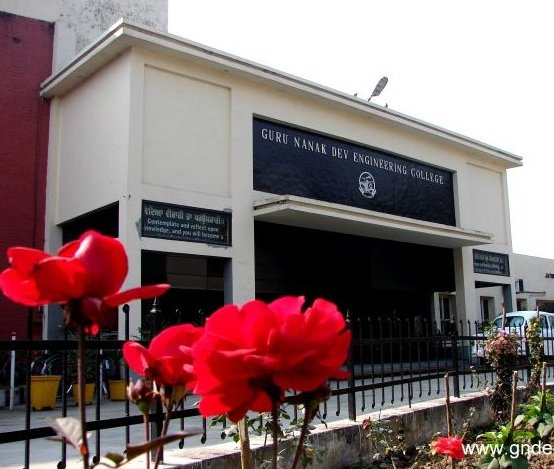
\includegraphics[scale=0.5]{images/gndec.jpg}
\caption{Guru Nanak Dev Engineering College}
\end{figure}
\hspace{-1.7em} I had my Six Weeks Industrial Training at TCC-Testing And Consultancy Cell, GNDEC Ludhiana. Guru Nanak Dev Engineering College was established by the Nankana
Sahib Education Trust Ludhiana. The Nankana Sahib Education Trust i.e NSET
was founded in memory of the most sacred temple of Sri Nankana Sahib, birth place
of Sri Guru Nanak Dev Ji. With the mission of Removal of Economic Backwardness
through Technology Shiromani Gurudwara Parbandhak Committee i.e SGPC started a
Poly technical was started in 1953 and Guru Nanak Dev Engineering College was established in 1956.\\

NSET resolved to uplift Rural areas by admitting 70\% 
of students from these rural
areas ever year. This commitment was made to nation on 8th April, 1956, the day
foundation stone of the college building was laid by Dr. Rajendra Prasad Ji, the First
President of India. The College is now ISO 9001:2000 certified.\\

The main goal of this institute is:\\
\begin{itemize}
\item To build and promote teams of experts in the upcoming specialisations.
\item To promote quality research and undertake research projects keeping in view their
relevance to needs and requirements of technology in local industry.
\item To achieve total financial independence.
\item To start online transfer of knowledge in appropriate technology by means of establishing multipurpose resource centres.
\end{itemize}
\section{Testing and Consutancy Cell}

My Six Weeks Institutional Training was done by me at TCC i.e Testing And
Consultancy Cell,
GNDEC Ludhiana under the guidance of Dr. H.S.Rai Dean Testing and Consultancy Cell.
Testing and Consultancy Cell was established in the year 1979 with a basic aim to produce
quality service for technical problems at reasonable and affordable rates as a service to society
in general and Engineering fraternity in particular.\\
\begin{figure}[ht]
\centering
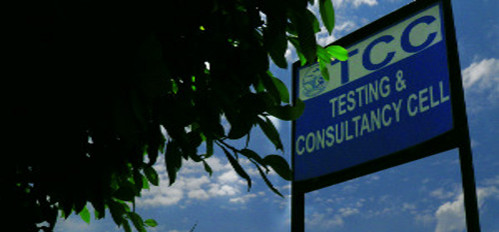
\includegraphics[scale=0.7]{images/aw.jpg}
\caption{Testing and Consultancy Cell}
\end{figure}
\hspace{-1.7em} 

Consultancy Services are being rendered by various Departments of the College to the
industry, Sate Government Departments and Entrepreneurs and are extended in the form of
expert advice in design, testing of materials \& equipment, technical surveys, technical audit,
calibration of instruments, preparation of technical feasibility reports etc.
This consultancy cell of the college has given a new dimension to the development
programmers of the College. Consultancy projects of over Rs. one crore are completed by the
Consultancy cell during financial year 2009-10. \\

Ours is a pioneer institute providing Consultancy Services in the States of Punjab, Haryana,
Himachal, J\&K and Rajasthan. Various Major Clients of the Consultancy Cell are as under:\\
\begin{itemize}
\item Northern Railway, Govt. of India
\item Indian Oil Corporation Ltd.
\item Larson \& Turbo.
\item Multi National Companies like AFCON \& PAULINGS.
\item Punjab Water Supply \& Sewage Board
\end{itemize}


\newpage
%\chapter{\LaTeX}
%\section{Introduction to \LaTeX}

\LaTeX, I had never heard about this term before doing this project,
but when I came to know about it's features, found it excellent. 
\LaTeX{} (pronounced /ˈleɪtɛk/, /ˈleɪtɛx/, /ˈlɑːtɛx/, or /ˈlɑːtɛk/) is a 
document markup language and document preparation system for the \TeX{} 
typesetting  program. Within the typesetting system, its name is styled 
as \LaTeX.

\image{0.9}{images/donald.png}{Donald Knuth, Inventor Of \TeX{} 
typesetting system}

Within the typesetting system, its name is styled as \LaTeX. The term 
\LaTeX{} refers only to the language in which documents are written, 
not to the editor used to write those documents. In order to create a 
document in \LaTeX, a .tex file must be created using some form of text 
editor. While most text editors can be used to create a \LaTeX{} document, 
a number of editors have been created specifically for working with \LaTeX.

\LaTeX{} is most widely used by mathematicians, scientists, 
engineers, philosophers, linguists, economists and other scholars in 
academia. As a primary or intermediate format, e.g., translating DocBook 
and other XML-based formats to PDF, \LaTeX{} is used because of the 
high quality of typesetting achievable by \TeX. The typesetting system 
offers programmable desktop publishing features and extensive facilities 
for automating most aspects of typesetting and desktop publishing, 
including numbering and cross-referencing, tables and figures, 
page layout and bibliographies.

\LaTeX{} is intended to provide a high-level language that
accesses the power of \TeX. \LaTeX{} essentially comprises a
collection of \TeX{} macros and a program to process \LaTeX documents. 
Because the \TeX{} formatting commands are very low-level, it is usually 
much simpler for end-users to use \LaTeX{}.


\subsection{Typesetting}
\LaTeX{} is based on the idea that authors should be able to focus on 
the content of what they are writing without being distracted by its 
visual presentation. In preparing a \LaTeX{} document, the author 
specifies the logical structure using familiar concepts such as 
chapter, section, table, figure, etc., and lets the \LaTeX{} system 
worry about the presentation of these structures. It therefore 
encourages the separation of layout from content while still allowing 
manual typesetting adjustments where needed. 

\begin{verbatim}
\documentclass[12pt]{article}
\usepackage{amsmath}
\title{\LaTeX}
\date{}
\begin{document}
  \maketitle 
  \LaTeX{} is a document preparation system 
  for the \TeX{} typesetting program.
   \par 
   $E=mc^2$
\end{document}
\end{verbatim}


\chapter{Introduction To Project}

% pending 
\section{Overview}
Design Reinforcement of Structures (DRB) is an open-source, free web-based software, developed by students of 
Testing and Consultancy Cell (TCC), under the guidance of Dr. H.S. Rai. This software is used to gives the 
Different views of structure of a building like Beams and Columns used to make a structure. This software can be used by Civil Engineers to view and anaylsis the strucure.

 The main task of this application is to get data as input from user and then it can compute 
the result and draw 2D views of the structure and user can download the views as a pdf format .
This software is structured by keeping in view that user of this software can be both 
a Civil Engineer or a simple man whose job is just to enter data to software 
in order that an engineer can analyze later from the result stability of the structure.
This software also provides the intermediate values for engineering student 
to deeply analyze the process of computation to be done in order to get output values.


The core part of DRB is implemented using JavaScript for processing, canvas for graphics and  jspdf.js for output file (PDF) generation, Angular.js 
for web interface. To provide the User Experience to the users, 
CSS and Bootstrap has been used.


My training being not based on particular language or technology, different type of open-source softwares and technologies are 
used in this project and many during my training which are not used in this 
project like Angular.js (for a declarative user interface and as front-end), Node.js (for server-side and managing databases).


%%%% This include existing system and will include user requirement
\section{The Existing System}
There are few existing systems for solving this particular problem like AutoCad but they don't have
following features required by our mentor. These system were not open source and free web based software 
that were need.


All exiting system suffers from at least one of the following system.  



{\bf {Limitations of previous system }}
\begin{itemize}
\item No batch mode 

\item Don't give output as PDF

\item They are costly ( AutoCad costs nearly 14,000 rupees )

\item They don't allow to download as pdf

\item They need installation and a lot of system resources 
 
\end{itemize}



\section{User Requirement Analysis} 
For User Requirement Analysis, users of this system have been asked about 
possible requirements that this software should have and we got following
resultant list of outputs-:
\begin{enumerate}
\item Generates the final output in the form of pdf
\item Provide on-line way to analysis so that individual does not have to 
install anything.
\item Save PDF in user PC in s/he favorite location
\item Make it work like batch mode. so, that user can give inputs 
together and relax.
\item Help B.Tech, M.Tech and Civil Engineer to analysis structure.
\item Automate calculation of modal force and modes.
\item Reduce the time for analysis.
\end{enumerate}


\section{Feasibility Analysis}
Feasibility analysis aims to uncover the strengths and weaknesses of 
a project. In its simplest term, the two criteria to judge feasibility 
are cost required and value to be attained. As such, a well-designed 
feasibility analysis should provide a historical background of the 
project, description of the project or service, details of the 
operations and management and legal requirements. Generally, feasibility 
analysis precedes technical development and project implementation. 
There is some feasibility factors by which we can determine that 
project is feasible or not:
\begin{itemize}
\item {\bf{Technical feasibility}}: Technological feasibility is carried 
out to determine whether the project has the capability, in terms of 
software, hardware, personnel to handle and fulfill the user 
requirements. This whole project is based on solving Mathematics equations for which we have used javaScript and to provide output we have used Canvas for providing the output and jspdf.js for pdf genaration and Angular.js for user interface and Node.js as backend. Technical feasibility of this project revolves around the technical boundaries and limitations jspdf.js and Angular.js. But as node.js is secure and structured server side framework, so these languages and technologies are perfect to design the software under this project. Design Reinforcement of Beam(DRB) is technically feasible as it is built up in Open 
Source Environment and thus it can be run on any Open Source platform.
\item {\bf{Economic feasibility}}: Economic analysis is the most 
frequently used method to determine the cost/benefit factor for 
evaluating the effectiveness of a new system. In this analysis we 
determine whether the benefit is gain according to the cost invested 
to develop the project or not. If benefits outweigh costs, only then 
the decision is made to design and implement the system. It is 
important to identify cost and benefit factors, which can be categorized 
as follows:
\begin{enumerate}
\item Development costs.
\item Operating costs.
\end{enumerate}
Design Reinforcement of Beam(DRB) Software is also Economically feasible with 0 Development 
and Operating Charges as it is developed in Angular.js framework, nade.js and jspdf.js  which is FOSS technology and the software is operated on Open 
Source platform.
\item {\bf{Operational feasibility}}: Operational feasibility is a measure 
of how well a project solves the problems, and takes advantage of the 
opportunities identified during scope definition and how it satisfies 
the requirements identified in the requirements analysis phase of system 
development. All the Operations performed in the software are very quick 
and satisfies all the reuirements. This project is also operational feasible as it automates the work of solving the problem of analysising the structures which not only saves time but also saves money as most of the work is done by Employees and M.Tech students is done by this software.
\end{itemize}




\section{Objective of Project}
Design Reinforcement of Beam(DRB) is a web based software and the 
main objectives of this project is to -:
\begin{enumerate}
\item To inspire M.Tech students to automate their work and do programming 
\item Perform most of difficult Calculation work.
\item Make it work like batch mode. so, that user can give inputs 
together and relax.
\item Help M.Tech and Civil Engineer to analysis structure.
\item Automatic calculation of modal force and modes.
\item Reduce the time for analysis.
\item Generates the final output in the form of graphics and also in pdf format.
\item Provide on-line way to analysis so that individual does not have to 
install anything.
\item User can download the views in pdf file anywhere.
\end{enumerate}

\chapter{PROJECT DESIGN}
\section{Software Requirement Analysis}

A Software Requirements Analysis for a software system is a complete 
description of the behavior of a system to be developed. It include functional Requirements
and Software Requirements. In addition to these, the SRS also contains 
non-functional requirements. Non-functional requirements are 
requirements which impose constraints on the design or implementation.
\begin{itemize}
\item{\bf Purpose}: Dynamic of structure is a web based software and the 
main purpose of this project is to:
\begin{enumerate}
\item Perform most of difficult Calculation work.
\item Make it work like batch mode. so, that user can give inputs 
together and relax.
\item Help M.Tech and Civil Engineer to analysis structure.
\item Automatic calculation of modal force and modes.
\item Reduce the time for analysis.
\item Provide on-line way to analysis so that individual does not have to 
install anything.
\end{enumerate}

\item{\bf Users of the System}
\begin{enumerate} 
\item Client : Clients are the end users that benefit from this software.
They just provide input and gets output in form of PDF.Client of this 
WEB Application can be of two types -:
\begin{enumerate}
\item Civil Engineer -: They have knowledge of working of procedure
and what input is being provided.
\item Layman -: They don't know anything about what's going on, their just 
work is to give input to system.   
 
\end{enumerate}
\end{enumerate}
\end{itemize}

\subsection{Functional Requirements}
\begin{itemize}
\item {\bf Specific Requirements}: This phase covers the whole requirements 
for the system. After understanding the system we need the input data 
to the system then we watch the output and determine whether the output 
from the system is according to our requirements or not. So what we have 
to input and then what we’ll get as output is given in this phase. This 
phase also describe the software and non-function requirements of the 
system.
\item {\bf Input Requirements of the System}
\begin{enumerate} 
\item Lenght of the baem
\item Width of the baem
\item Breadth of the baem
\item Diameter of the Main Bar
\item Diameter of the Anchor Bar
\item Diameter of the Stirrup Bar
\item Spacing between the stirrups
\end{enumerate}
\vskip 0.5cm
\item {\bf Output Requirements of the System}
\begin{enumerate} 
\item Calculating and viewing graphical views of the result.
\item Genrating output PDF.
\end{enumerate}
\vskip 0.5cm
\item {\bf Software Requirements}
\begin{enumerate} 
\item Programming language: JavaScript
\item software: \LaTeX{}
\item Libraries: jspdf.js
\item Backend: Node.js
\item Framework: Angular.js, Express.js and Bootstrap
\item Web Languages: Html, JavaScript, CSS
\item Database: MongoDB
\item Text Editor: Atom
\item Operating System: Ubuntu 14.04 or up
\item Revision System: Git

\end{enumerate}
\vskip 0.5cm
\subsection{Non functional requirements}
\begin{enumerate} 
\item Scalability: System should be able to handle a number of users. 
For e.g., handling around thousand users at the same time.
\item Usability: Simple user interfaces that a layman can understand.
\item Speed: Processing input should be done in reasonable time
 i.e. we can say maximum 24 hrs.
\end{enumerate}
\end{itemize}




\section{Dependencies}
Dependencies include softwares or framework that need to be installed for 
proper working of this software.

\begin{enumerate} 
\item Programming language: JavaScript
\item Software: \LaTeX{}
\item Framework: Angular.js and Express.js
\item Operating System: Any on which above dependencies can be installed
\end{enumerate}







\newpage
\chapter{DEVELOPMENT AND IMPLEMENTATION}
\section{Angular.js} 
\begin{figure}[h]
\centering 
\includegraphics[scale=0.3]{images/Angular.png}
\caption{Angular.js logo}
\end{figure}
\noindent AngularJS is a structural framework for dynamic web apps. It lets you use HTML as your template language and lets you extend HTML's syntax to express your application's components clearly and succinctly. Angular's data binding and dependency injection eliminate much of the code you would otherwise have to write. And it all happens within the browser, making it an ideal partner with any server technology.

Angular is not a single piece in the overall puzzle of building the client-side of a web application. It handles all of the DOM and AJAX glue code you once wrote by hand and puts it in a well-defined structure. This makes Angular opinionated about how a CRUD (Create, Read, Update, Delete) application should be built. But while it is opinionated, it also tries to make sure that its opinion is just a starting point you can easily change.

\begin{figure}[h]
\centering 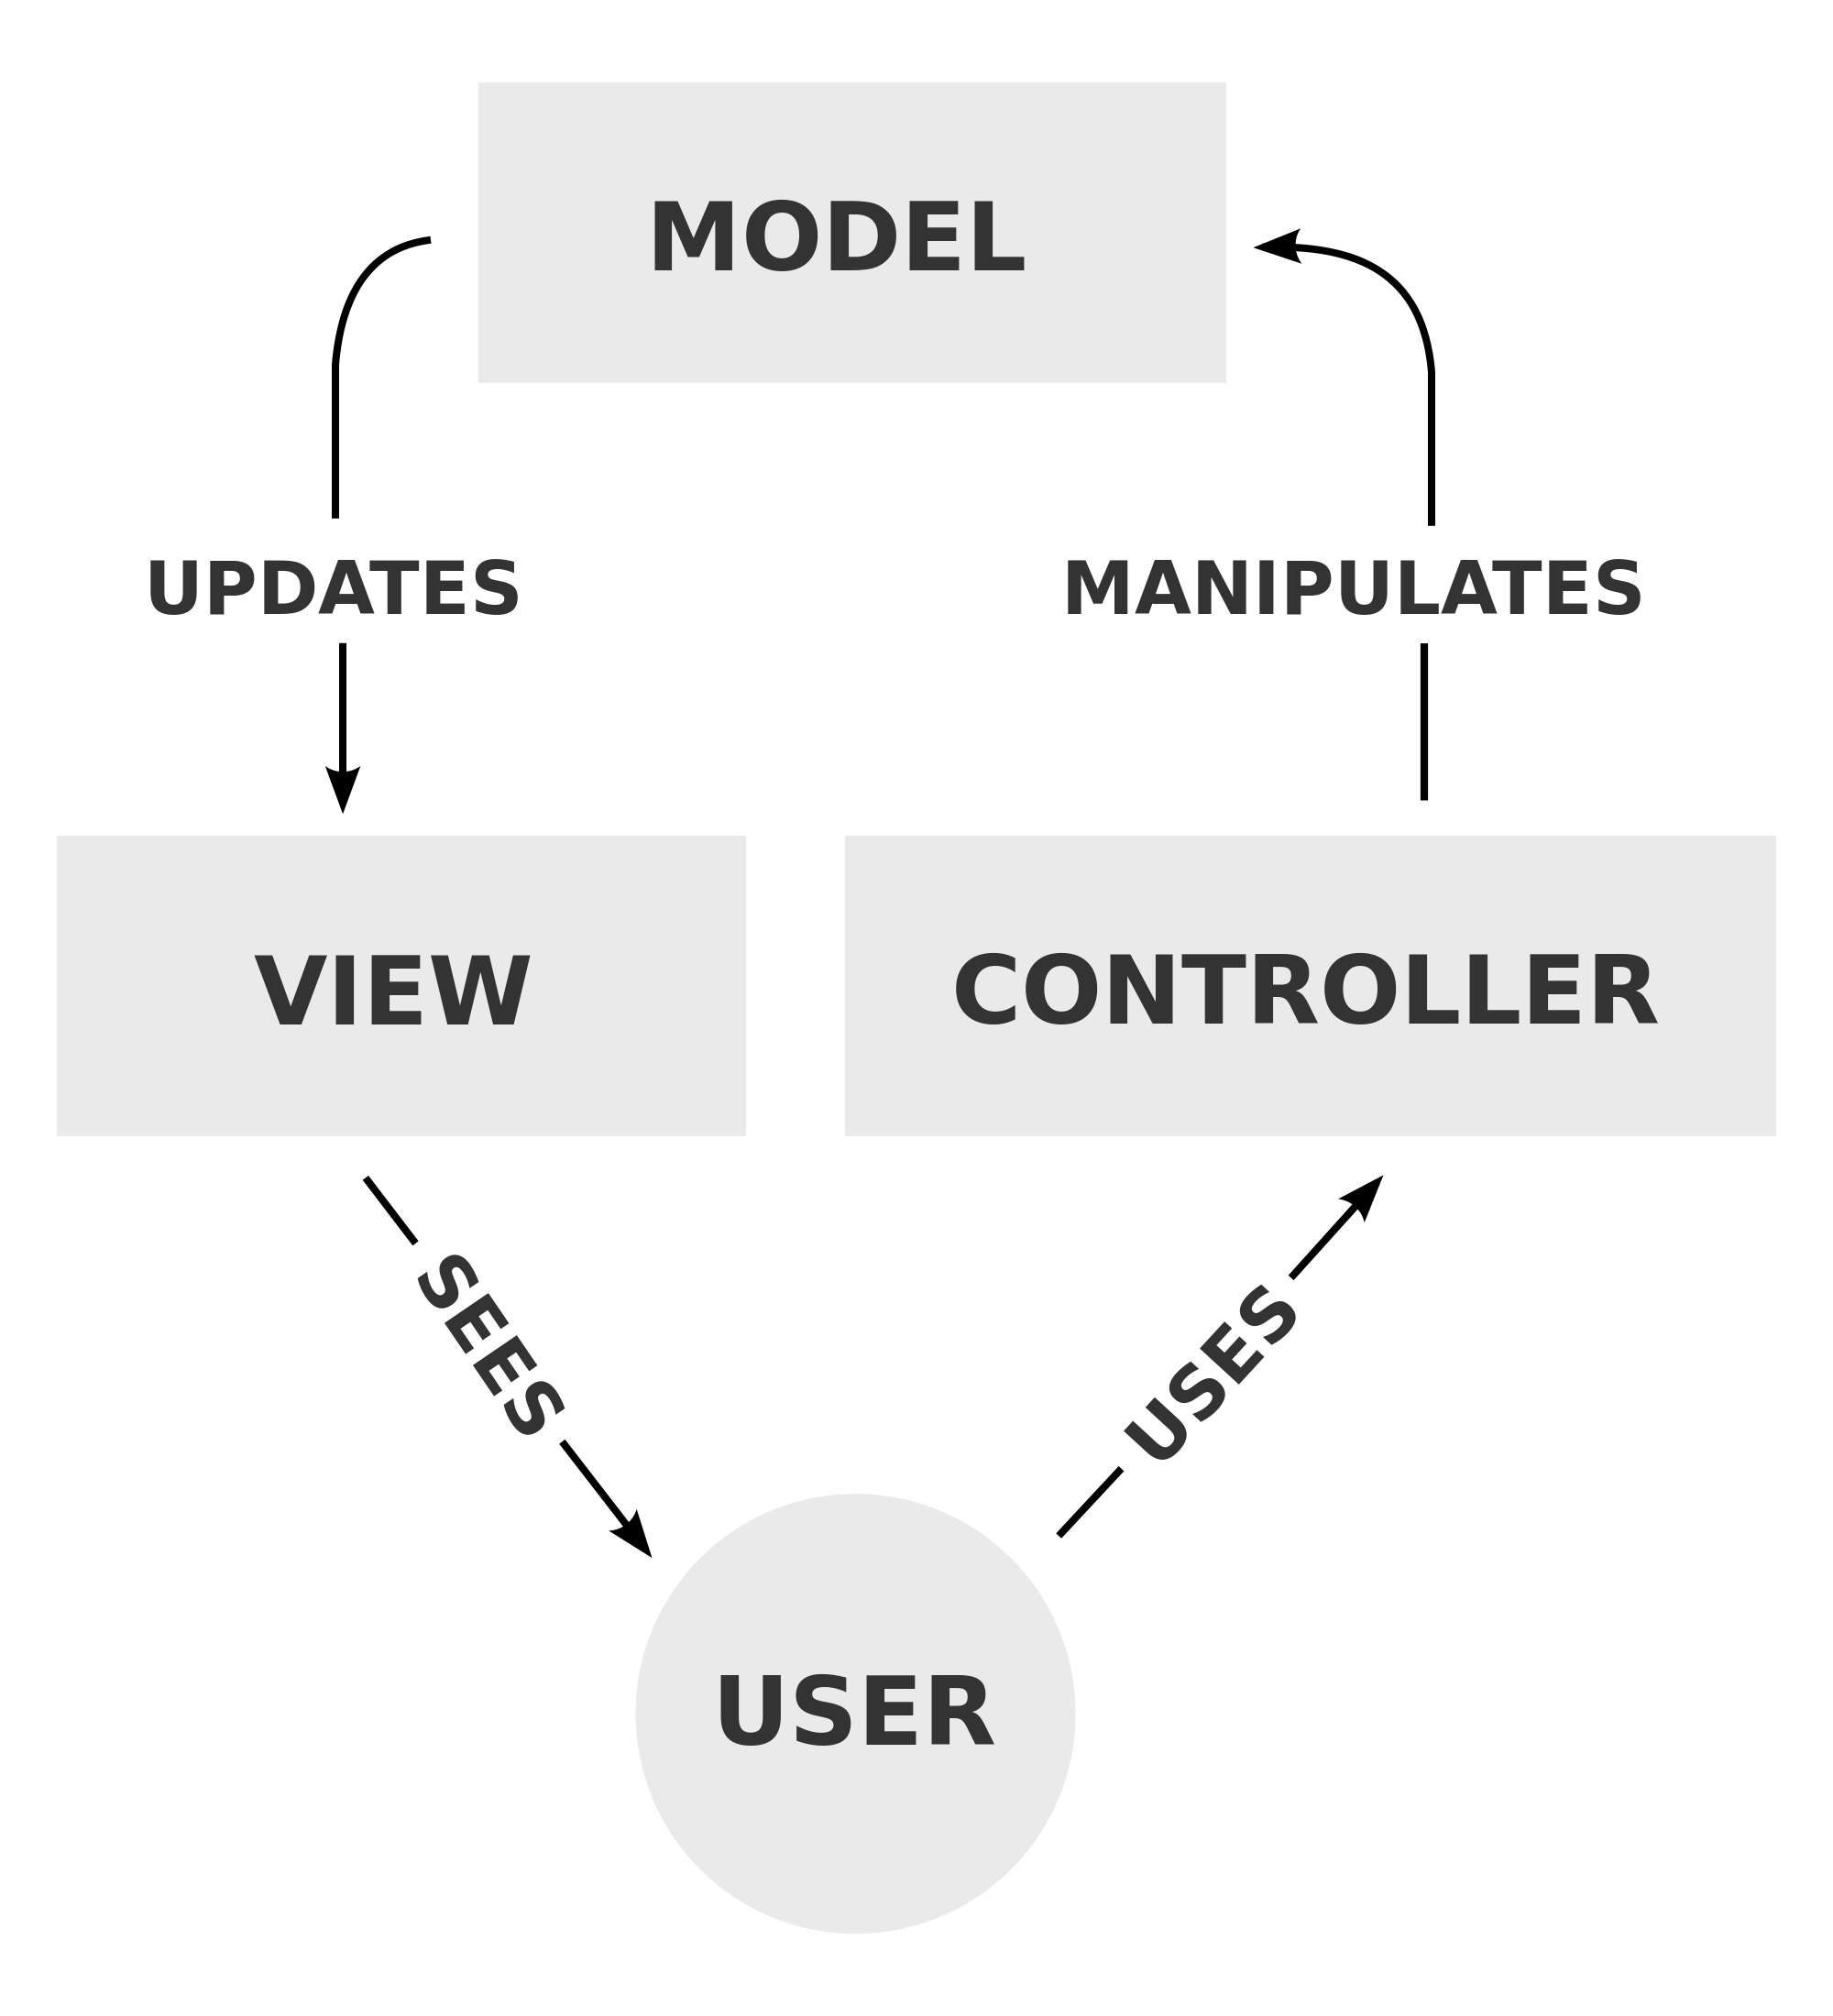
\includegraphics[scale=0.1]{images/mvc.png}
\caption{Model View Controller}
\end{figure}

\subsection{Features of Angular}
\begin{itemize}
\item It is a very good idea to decouple DOM manipulation from app logic. This dramatically improves the testability of the code.
\item It is a really, really good idea to regard app testing as equal in importance to app writing. Testing difficulty is dramatically affected by the way the code is structured.
\item It is an excellent idea to decouple the client side of an app from the server side. This allows development work to progress in parallel, and allows for reuse of both sides.
\item It is very helpful indeed if the framework guides developers through the entire journey of building an app: From designing the UI, through writing the business logic, to testing.
\item It is always good to make common tasks trivial and difficult tasks possible.
\end{itemize}



\section[Front End Languages and Framework]{Front End Languages 
and Framework \footnote{ Used in project but not by me accept 
basic HTML}}

Front End languages are language that are used to give better user experince and user interface. These mainly include HTML, CSS, Javascript. Some Frameforks like Bootstrap are also used with these basic languages.
\subsection{HTML}

\begin{figure}[h]
\centering 
\includegraphics[scale=0.05]{images/HTML.png}
\caption{HTML5 logo}
\end{figure}
HyperText Markup Language, commonly referred to as HTML, is the standard markup language used to create web pages. Along with CSS, and JavaScript, HTML is a cornerstone technology, used by most websites to create visually engaging webpages, user interfaces for web applications, and user interfaces for many mobile applications. Web browsers can read HTML files and render them into visible or audible web pages. HTML describes the structure of a website semantically along with cues for presentation, making it a markup language, rather than a programming language.


HTML elements form the building blocks of all websites. HTML allows images and objects to be embedded and can be used to create interactive forms. It provides a means to create structured documents by denoting structural semantics for text such as headings, paragraphs, lists, links, quotes and other items.

\begin{verbatim}
<!DOCTYPE html>
<html>
  <head>
    <title>This is a title</title>
  </head>
  <body>
    <p>Hello world!</p>
  </body>
</html>

\end{verbatim}


\subsection{CSS}

\begin{figure}[h]
\centering 
\includegraphics[scale=0.50]{images/CSS.jpg}
\caption{CSS logo}
\end{figure}
Cascading Style Sheets (CSS) is a style sheet language used for describing the presentation of a document written in a markup language.Although most often used to set the visual style of web pages and user interfaces written in HTML and XHTML, the language can be applied to any XML document, including plain XML, SVG and XUL, and is applicable to rendering in speech, or on other media. Along with HTML and JavaScript, CSS is a cornerstone technology used by most websites to create visually engaging webpages, user interfaces for web applications, and user interfaces for many mobile applications.


CSS is designed primarily to enable the separation of document content from document presentation, including aspects such as the layout, colors, and fonts. This separation can improve content accessibility, provide more flexibility and control in the specification of presentation characteristics, enable multiple HTML pages to share formatting by specifying the relevant CSS in a separate .css file, and reduce complexity and repetition in the structural content, such as semantically insignificant tables that were widely used to format pages before consistent CSS rendering was available in all major browsers. CSS makes it possible to separate presentation instructions from the HTML content in a separate file or style section of the HTML file. For each matching HTML element, it provides a list of formatting instructions

\begin{verbatim}
p {
    color: red;
    text-align: center;
}
\end{verbatim}

\subsection{Javascript}
\begin{figure}[h]
\centering 
\includegraphics[scale=0.3]{images/JS.png}
\caption{Javascript logo}
\end{figure}
JavaScript (/ˈdʒɑːvəˌskrɪpt/) is a high-level, dynamic, untyped, and interpreted programming language. It has been standardized in the ECMAScript language specification. Alongside HTML and CSS, it is one of the three essential technologies of World Wide Web content production; the majority of websites employ it and it is supported by all modern web browsers without plug-ins. JavaScript is prototype-based with first-class functions, making it a multi-paradigm language, supporting object-oriented, imperative, and functional programming styles. It has an API for working with text, arrays, dates and regular expressions, but does not include any I/O, such as networking, storage or graphics facilities, relying for these upon the host environment in which it is embedded.

\subsection{BootStrap}
\begin{figure}[h]
\centering 
\includegraphics[scale=0.2]{images/boot.png}
\caption{BootStrap logo}
\end{figure}

Bootstrap is a free and open-source collection of tools for creating websites and web applications. It contains HTML and CSS-based design templates for typography, forms, buttons, navigation and other interface components, as well as optional JavaScript extensions. It aims to ease the development of dynamic websites and web applications.

Bootstrap is a front end framework, that is, an interface for the user, unlike the server-side code which resides on the "back end" or server.


\section{Shell Scripting}
Normally shells are interactive. It means shell accept command from you (via keyboard) and execute them. But if you use command one by one (sequence of 'n' number of commands) , the you can store this sequence of command to text file and tell the shell to execute this text file instead of entering the commands. This is know as shell script.
Shell script defined as series of command written in plain text file. Shell script is just like batch file is MS-DOS but have more power than the MS-DOS batch file.
why to Write Shell Script ?
\begin{enumerate} 
\item Shell script can take input from user, file and output them on screen.
\item Useful to create our own commands.
\item Save lots of time.
\item To automate some task of day-to-day life.
\item System Administration part can be also automated.
\end{enumerate} 
{ \bf Execute your script as syntax:}
\begin{verbatim}
chmod 755 your-script-name
sh your-script-name
./your-script-name
\end{verbatim}

\section{Introduction to \LaTeX}

\LaTeX, I had never heard about this term before doing this project,
but when I came to know about it's features, found it excellent. 
\LaTeX{} (pronounced /ˈleɪtɛk/, /ˈleɪtɛx/, /ˈlɑːtɛx/, or /ˈlɑːtɛk/) is a 
document markup language and document preparation system for the \TeX{} 
typesetting  program. Within the typesetting system, its name is styled 
as \LaTeX.

\image{0.9}{images/donald.png}{Donald Knuth, Inventor Of \TeX{} 
typesetting system}

Within the typesetting system, its name is styled as \LaTeX. The term 
\LaTeX{} refers only to the language in which documents are written, 
not to the editor used to write those documents. In order to create a 
document in \LaTeX, a .tex file must be created using some form of text 
editor. While most text editors can be used to create a \LaTeX{} document, 
a number of editors have been created specifically for working with \LaTeX.

\LaTeX{} is most widely used by mathematicians, scientists, 
engineers, philosophers, linguists, economists and other scholars in 
academia. As a primary or intermediate format, e.g., translating DocBook 
and other XML-based formats to PDF, \LaTeX{} is used because of the 
high quality of typesetting achievable by \TeX. The typesetting system 
offers programmable desktop publishing features and extensive facilities 
for automating most aspects of typesetting and desktop publishing, 
including numbering and cross-referencing, tables and figures, 
page layout and bibliographies.

\LaTeX{} is intended to provide a high-level language that
accesses the power of \TeX. \LaTeX{} essentially comprises a
collection of \TeX{} macros and a program to process \LaTeX documents. 
Because the \TeX{} formatting commands are very low-level, it is usually 
much simpler for end-users to use \LaTeX{}.


\subsection{Typesetting}
\LaTeX{} is based on the idea that authors should be able to focus on 
the content of what they are writing without being distracted by its 
visual presentation. In preparing a \LaTeX{} document, the author 
specifies the logical structure using familiar concepts such as 
chapter, section, table, figure, etc., and lets the \LaTeX{} system 
worry about the presentation of these structures. It therefore 
encourages the separation of layout from content while still allowing 
manual typesetting adjustments where needed. 

\begin{verbatim}
\documentclass[12pt]{article}
\usepackage{amsmath}
\title{\LaTeX}
\date{}
\begin{document}
  \maketitle 
  \LaTeX{} is a document preparation system 
  for the \TeX{} typesetting program.
   \par 
   $E=mc^2$
\end{document}
\end{verbatim}



\section{Introduction to Node.js}
\begin{figure}[h]
\centering 
\includegraphics[scale=0.13]{images/Node.png}
\caption{Node.js logo}
\end{figure}
\noindent Node.js is a server-side platform built on Google Chrome's JavaScript Engine (V8 Engine). Node.js was developed by Ryan Dahl in 2009 and its latest version is v0.10.36.

Node.js is an open source, cross-platform runtime environment for developing server-side and networking applications. Node.js applications are written in JavaScript, and can be run within the Node.js runtime on OS X, Microsoft Windows, and Linux.

Node.js also provides a rich library of various JavaScript modules which simplifies the development of web applications using Node.js to a great extent.

\subsection{Features of Node.js}
\begin{itemize}
\item Asynchronous and Event Driven \− All APIs of Node.js library are asynchronous, that is, non-blocking. It essentially means a Node.js based server never waits for an API to return data.
\item Very Fast \− Being built on Google Chrome's V8 JavaScript Engine, Node.js library is very fast in code execution.
\item Single Threaded but Highly Scalable \− Node.js uses a single threaded model with event looping.
\item No Buffering \− Node.js applications never buffer any data. These applications simply output the data in chunks.
\end{itemize}
\subsection{Installation of Node.js}
Installation of Node.js is very easy. To install Node.js,
type the following commands:\\

	\$ curl -sL https://deb.nodesource.com/setup-6.x -o nodesource-setup.sh\\


	\$ nano nodesource-setup.sh\\


	\$ sudo apt-get install nodejs\\


	\$ sudo apt-get install build-essential\\


	\$ sudo apt-get install npm \\

\noindent This will install the node on your system.

\noindent \subsection{Creating Node.js project} The source code that you would write in a source file is simply javascript. The Node.js interpreter interprets and executes your javascript code.
\begin{itemize}
\item {\bf{Import Required Module}} We use the require directive to load the http module and store the returned HTTP instance into an http variable as follows −
\begin{figure}[h]
\centering 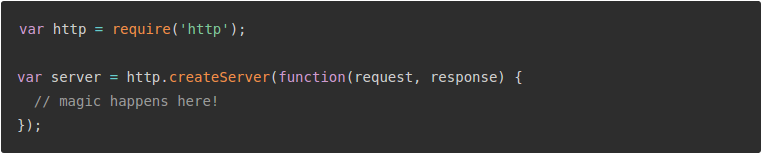
\includegraphics[scale=0.5]{images/1.png}
\caption{creating nodejs project.js}
\end{figure}

\item {\bf{Create Server}} We use the created http instance and call http.createServer() method to create a server instance and then we bind it at port 8081 using the listen method associated with the server instance. Pass it a function with parameters request and response. Write the sample implementation to always return "Hello World".
\begin{figure}[h]
\centering 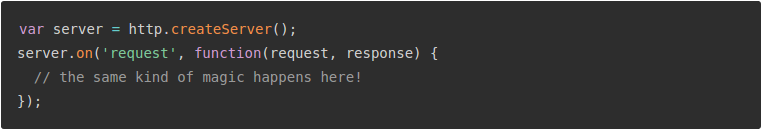
\includegraphics[scale=0.5]{images/2.png}
\caption{creating server.js}
\end{figure}

\item {\bf{Testing Request \& Response}} Let's put step 1 and 2 together in a file called main.js and start our HTTP server. Now execute the main.js to start the server as follows −

	\$ node main.js \\

\end{itemize}
\subsection{Starting Server in node.js}
In order to check your successful Node installation we can try out a very simple console command\\

	\$ node server.js \\

\noindent This command will start server in your console.\\

\subsection{Database setup}
To work with the database, you first need to create a connection. In this section of the tutorial, we will be using MongoDB’s native Node.js driver to create the connection with the MongoDB server. To install the mongodb native drivers, use the npm command to install the mongodb module. After that, run the following command in your project directory.

	\$ npm install mongodb \\

\begin{itemize}
\item npm is a package manager that provides a central repository for custom open source modules for Node.js and JavaScript. npm makes it simple to manage modules, their versions and distribution. As shown in the preceding paragraph, the npm install command was used to install the required module in our project.

\item Load the mongodb module : We used require to load the mongodb module in our code. mongodb module represents the native mongodb drivers for Node.js.

\item Defining the URL we need to connect to: We need to know where our mongodb server is running. The url represents the location where the mongodb server instance is running such that we can connect to it. The url contains the database name to which we intend to connect.

\item Connect to the database: Let’s use the MongoClient interface to connect to the database. In the callback we get error or the db object. We use the db object in order to communicate with the database.

\end{itemize}


\section{Introduction to MongoDB}
\begin{figure}[h]
\centering 
\includegraphics[scale=1]{images/mongoPic.png}
\caption{MongoDB logo}
\end{figure}
\noindent MongoDB is a cross-platform, document oriented database that provides, high performance, high availability, and easy scalability. MongoDB works on concept of collection and document.

Database is a physical container for collections. Each database gets its own set of files on the file system. A single MongoDB server typically has multiple databases.

Collection is a group of MongoDB documents. It is the equivalent of an RDBMS table. A collection exists within a single database. Collections do not enforce a schema. Documents within a collection can have different fields. Typically, all documents in a collection are of similar or related purpose.

A document is a set of key-value pairs. Documents have dynamic schema. Dynamic schema means that documents in the same collection do not need to have the same set of fields or structure, and common fields in a collection's documents may hold different types of data.

\begin{figure}[h]
\centering 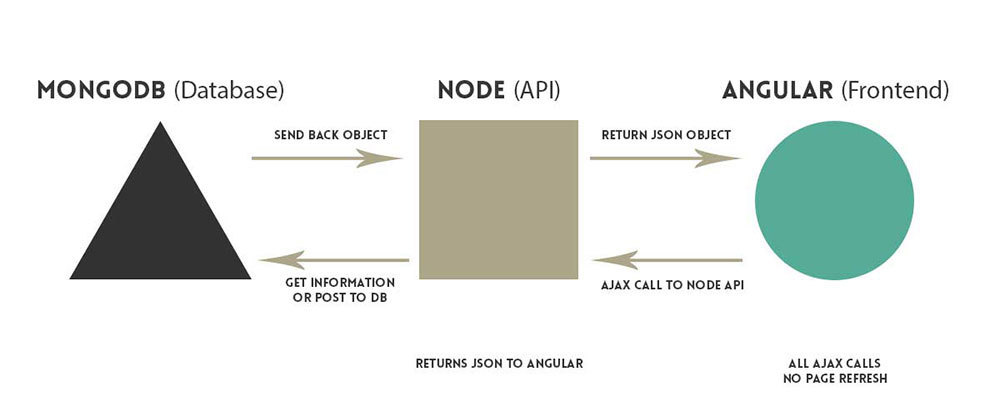
\includegraphics[scale=1]{images/mongodb.jpg}
\caption{Mean Model}
\end{figure}

\subsection{Advantages of MongnoDB}
\begin{itemize}
\item Schema less − MongoDB is a document database in which one collection holds different documents. Number of fields, content and size of the document can differ from one document to another.
\item Deep query-ability. MongoDB supports dynamic queries on documents using a document-based query language that's nearly as powerful as SQL.
\item Uses internal memory for storing the (windowed) working set, enabling faster access of data.
\item Conversion/mapping of application objects to database objects not needed.
\end{itemize}

\subsection{Why to use MongnoDB}
\begin{itemize}
\item Document Oriented Storage − Data is stored in the form of JSON style documents.
\item Index on any attribute.
\item Replication and high availability.
\item Auto-sharding
\end{itemize}

\subsection{Where to use MongnoDB}
\begin{itemize}
\item Big Data
\item Content Management and Delivery
\item Mobile and Social Infrastructure
\item User Data Management
\end{itemize}

\subsection{Installation of MongoDB}
Doxygen can be installed using following commands:\\

\hspace{4pt} \$ sudo apt-key adv --keyserver hkp://keyserver.ubuntu.com:80 --recv 0C49F3730359A14518585931BC711F9BA15703C6

\hspace{4pt} \$ sudo apt-get update

\hspace{4pt} \$ sudo apt-get install -y mongodb-org

\hspace{4pt} \$ sudo service mongod start



\section{Introduction to Github}
\begin{figure}[!ht]
\centering

\includegraphics[width=0.3\textwidth]{images/github}                   
\caption{Github Logo}
\hspace{-1.5em}
\end{figure}
\leavevmode\\
GitHub is a Git repository web-based hosting service which offers all of the functionality of Git as well as adding many of its own features. Unlike Git which is strictly a command-line tool, Github provides a web-based graphical interface and desktop as well as mobile integration. It also provides access control and several collaboration features such as wikis, task management, and bug tracking and feature requests for every project.\\

GitHub offers both paid plans for private repto handle everything from small to very large projects with speed and efficiency. ositories, and free accounts, which are usually used to host open source software projects. As of 2014, Github reports having over 3.4 million users, making it the largest code host in the world.\\

GitHub has become such a staple amongst the open-source development community that many developers have begun considering it a replacement for a conventional resume and some employers require applications to provide a link to and have an active contributing GitHub account in order to qualify for a job.\\

The Git feature that really makes it stand apart from nearly every
other Source Code Management (SCM) out there is its branching model.\\
\\
Git allows and encourages you to have multiple local branches that can
be entirely independent of each other. The creation, merging, and
deletion of those lines of development takes seconds.\\ \\
This means that you can do things like:
\begin{itemize}
\item Frictionless Context Switching.\\ Create a branch to try out an
idea, commit a few times, switch back to where you branched from,
apply a patch, switch back to where you are experimenting, and merge
it in.
\item Role-Based Code lines. \\ Have a branch that always contains only
what goes to production, another that you merge work into for testing,
and several smaller ones for day to day work.
\item Feature Based Work flow. \\ Create new branches for each new
feature you're working on so you can seamlessly switch back and forth
between them, then delete each branch when that feature gets merged
into your main line.
\item Disposable Experimentation.\\  Create a branch to experiment in,
realize it's not going to work, and just delete it - abandoning the
work—with nobody else ever seeing it (even if you've pushed other
branches in the meantime).
\end{itemize}
Notably, when you push to a remote repository, you do not have to push
all of your branches. You can choose to share just one of your
branches, a few of them, or all of them. This tends to free people to
try new ideas without worrying about having to plan how and when they
are going to merge it in or share it with others.\\ \\
There are ways to accomplish some of this with other systems, but the
work involved is much more difficult and error-prone. Git makes this
process incredibly easy and it changes the way most developers work
when they learn it.

\subsection{What is Git?}
\begin{figure}[!ht]
\centering

\includegraphics[width=0.3\textwidth]{images/git}                   
\caption{Git Logo}
\hspace{-1.5em}
\end{figure}
Git is a distributed revision control and source code management (SCM) system with an emphasis on speed, data integrity, and support for distributed, non-linear workflows. Git was initially designed and developed by Linus Torvalds for Linux kernel development in 2005, and has since become the most widely adopted version control system for software development.\\

As with most other distributed revision control systems, and unlike most client–server systems, every Git working directory is a full-fledged repository with complete history and full version-tracking capabilities, independent of network access or a central server. Like the Linux kernel, Git is free and open source software distributed under the terms of the GNU General Public License version 2 to handle everything from small to very large projects with speed and efficiency.\\

Git is easy to learn and has a tiny footprint with lightning fast performance. It outclasses SCM tools like Subversion, CVS, Perforce, and ClearCase with features like cheap local branching, convenient staging areas, and multiple workflows.\\

\subsection{Installation of Git}

Installation of git is a very easy process.
The current git version is: 2.0.4.
Type the commands in the terminal:\\\\
\emph{
\$ sudo apt-get update\\\\
\$ sudo apt-get install git\\\\}
This will install the git on your pc or laptop.

\subsection{Various Git Commands}

Git is the open source distributed version control system that facilitates GitHub activities on your laptop or desktop. The commonly used Git command line instructions are:-\\

\subsubsection{Create Repositories}
Start a new repository or obtain from an exiting URL

\begin{description}

\item [\$ git init [ project-name]]\\
Creates a new local repository with the specified name
\item [\$ git clone [url]]\\
Downloads a project and its entire version history\\

\end{description}


\subsubsection{Make Changes}
Review edits and craft a commit transaction

\begin{description}

\item [\$ git status] \leavevmode \\
Lists all new or modified files to be committed

\item [\$ git diff] \leavevmode \\
Shows file differences not yet staged

\item [\$ git add [file]]\\
Snapshots the file in preparation for versioning

\item [\$ git reset [file]]\\
Unstages the file, but preserve its contents

\item [\$ git commit -m \"[descriptive message]\"]\\
Records file snapshots permanently in version history\\

\end{description}


\subsubsection{Group Changes}
Name a series of commits and combine completed efforts

\begin{description}

\item [\$ git branch] \leavevmode \\
Lists all local branches in the current repository

\item [\$ git branch [branch-name]]\\
Creates a new branch

\item [\$ git checkout [branch-name]]\\
Switches to the specified branch and updates the working directory

\item [\$ git merge [branch]]\\
Combines the specified branch’s history into the current branch

\item [\$ git branch -d [branch-name]]\\
Deletes the specified branch\\

\end{description}


\subsubsection{Save Fragments}
Shelve and restore incomplete changes

\begin{description}

\item [\$ git stash] \leavevmode \\
Temporarily stores all modified tracked files

\item [\$ git stash pop] \leavevmode \\
Restores the most recently stashed files

\item [\$ git stash list] \leavevmode \\
Lists all stashed changesets

\item [\$ git stash drop] \leavevmode \\
Discards the most recently stashed changeset\\

\end{description}


\subsubsection{Synchronize Changes}
Register a repository bookmark and exchange version history

\begin{description}

\item [\$ git fetch [bookmark]]\\
Downloads all history from the repository bookmark

\item [\$ git merge [bookmark]/[branch]]\\
Combines bookmark’s branch into current local branch

\item [\$ git push [alias][branch]]\\
Uploads all local branch commits to GitHub

\item [\$ git pull] \leavevmode \\
Downloads bookmark history and incorporates changes

\end{description}




\section{Implementation}
Development of DRB started with development in phases which focus on particular need of project.
Various phases and their detail are given below -:
\begin{itemize}
\item Phase I : \\
	During Phase I, we wrote code in JavaScript to compute all the required output variable.
We use different controllers for the application. Controller named BeamControl fetch the data from the user and perform operations and gives out required result.
\item Phase II (\LaTeX{}) : \\
	During Phase II, we wrote code in JavaScript to compute all the required output variable.
We use different controllers for the application. Controller named BeamControl fetch the data from the user and perform operations and gives out required result.
	
\item Phase III : \\
	During phase III, we provided web interface to this software using Django. Djanog was used
	to get input from user and write input.sage file for particular user then civil.sh 
	is called by passing name of user directory to it and then get output PDF.
\item Phase IV : \\
	During phase IV, we improved the code structure and added additional 
	functionality like sending PDF as email and accepting input as CSV file.
	Finally, the UI was improved and made responsive.
\item Phase V : \\
During phase V, we tested the software for various conditions and then applied required error control and messaging 
mechanism. initialfile.py file was created to save software from problem of server restart which can causes processing user request to stop. so, that 
the interrupted request of user can be restart and send PDF.
\item Phase VI-: \\ 
During final phase, we documented the project( developers documentation and README.md) using doxygen and wrote the report for this software.    
\end{itemize}     

\begin{figure}[H] 
\centering 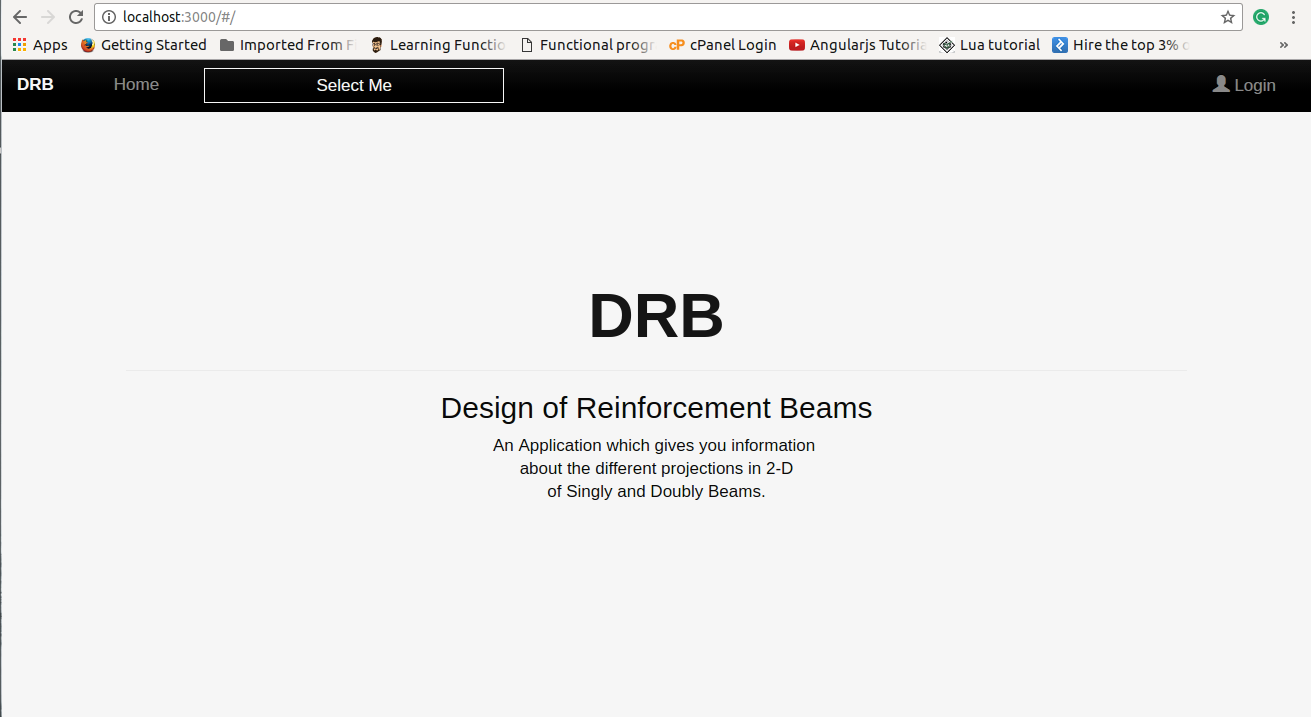
\includegraphics[scale=0.32]{images/output/screen1.png}
\caption{Home page of DRB}
\label{fig:1}
\end{figure}
This is the first interface that is shown to the user. This is the Home page.
It brings a nice UI to get input from user about the Number of storeys and 
some factor affecting the structure. It also provides the user some 
additional features as an aid like moving to specific operations the user want to do. There is an icon of logo i.e DRB which directs the user to home. There is also an login icon for user to login from different clients like gmail and facebook.\ref{fig:1}
\begin{figure}[H] 
\centering 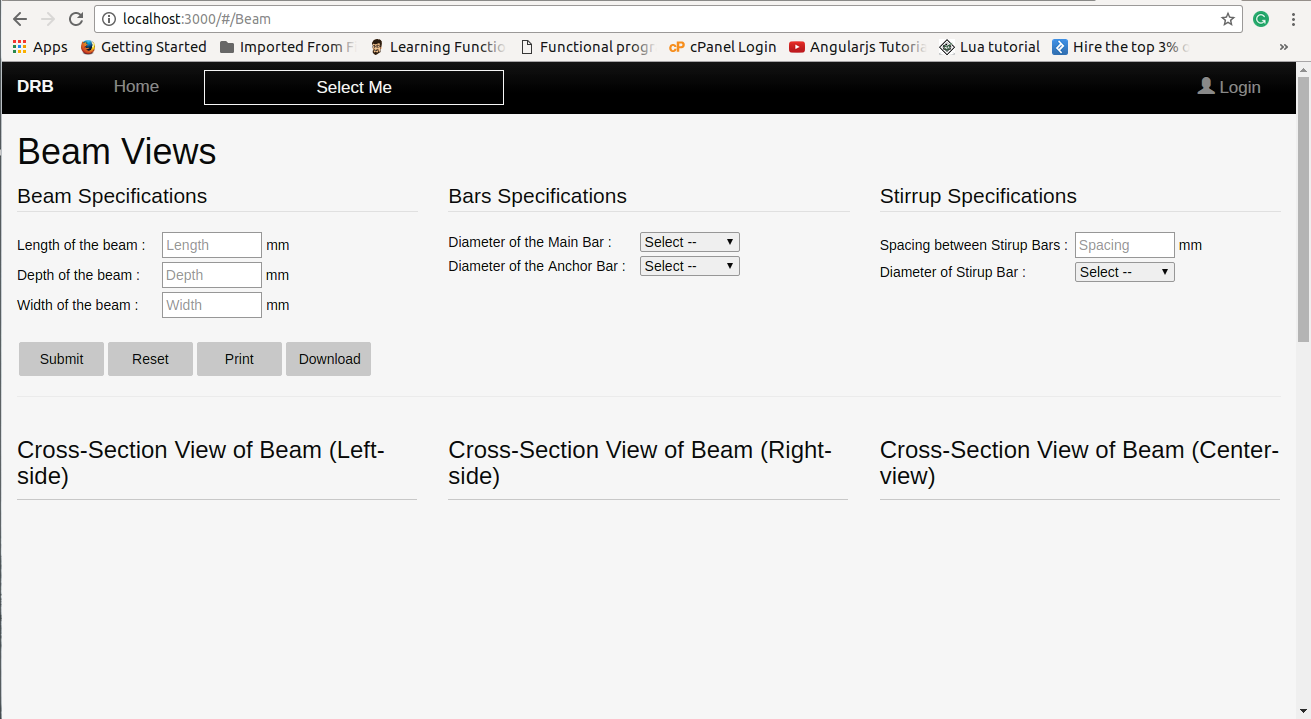
\includegraphics[scale=0.32]{images/output/screen2.png}
\caption{Beam Views}
\label{fig:2}
\end{figure}  


After filling the required data click the 'Submit' button on the page, Different views are drawn under the specific places.\ref{fig:2}

\begin{figure}[H] 
\centering 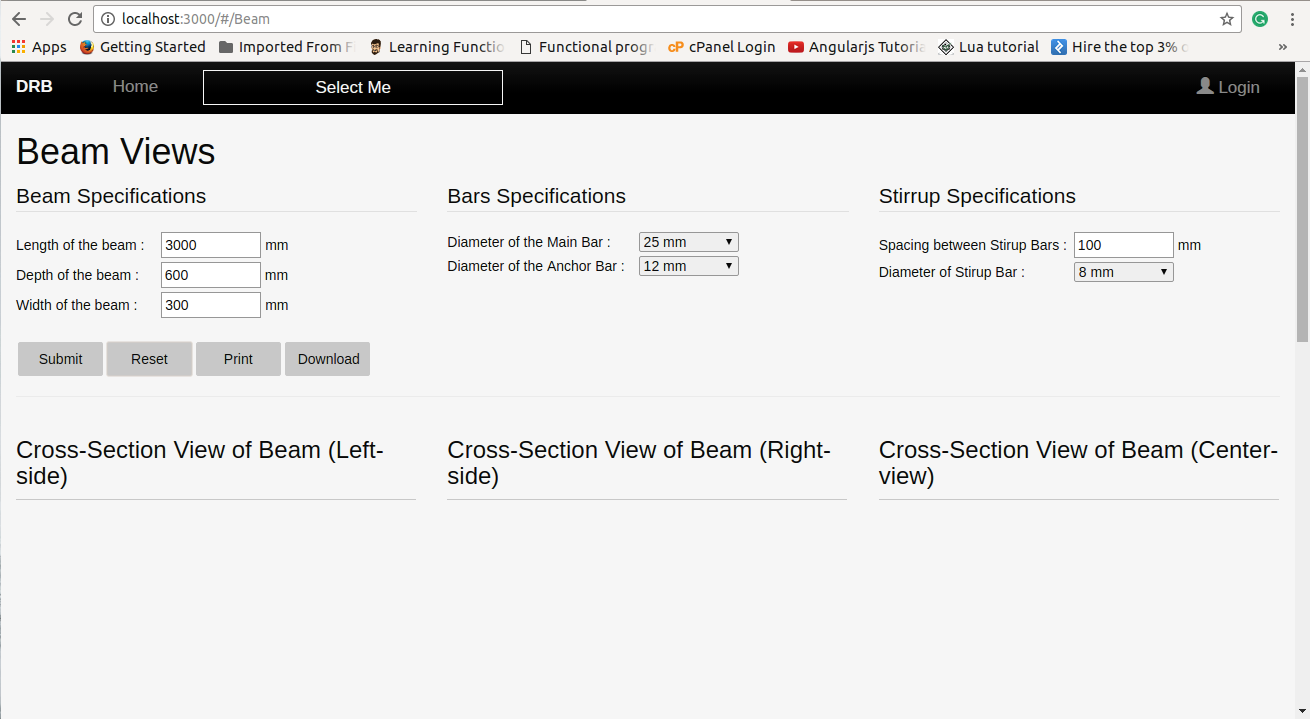
\includegraphics[scale=0.32]{images/output/screen3.png}
\caption{filling values}
\label{fig:3}
\end{figure}

After filling certain values.\ref{fig:3}

\begin{figure}[H] 
\centering 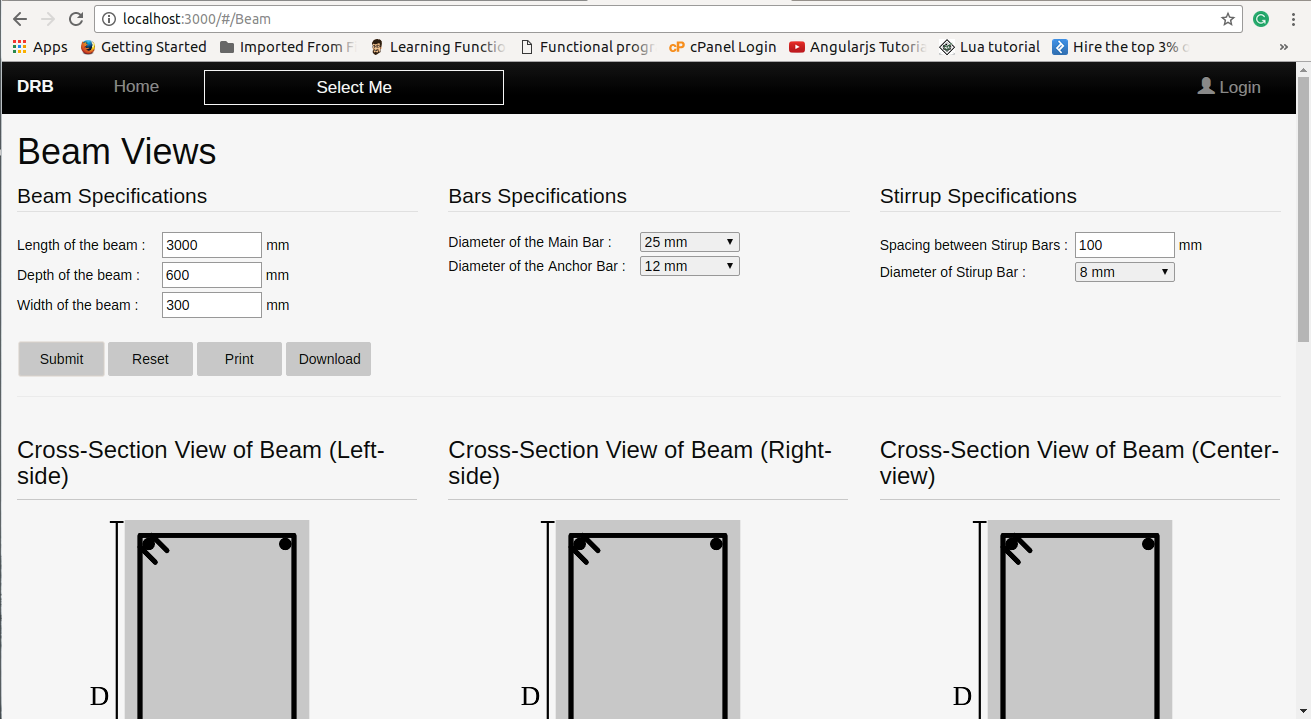
\includegraphics[scale=0.31]{images/output/screen4.png}
\caption{resulting view}
\label{fig:4}
\end{figure}

\begin{figure}[H] 
\centering 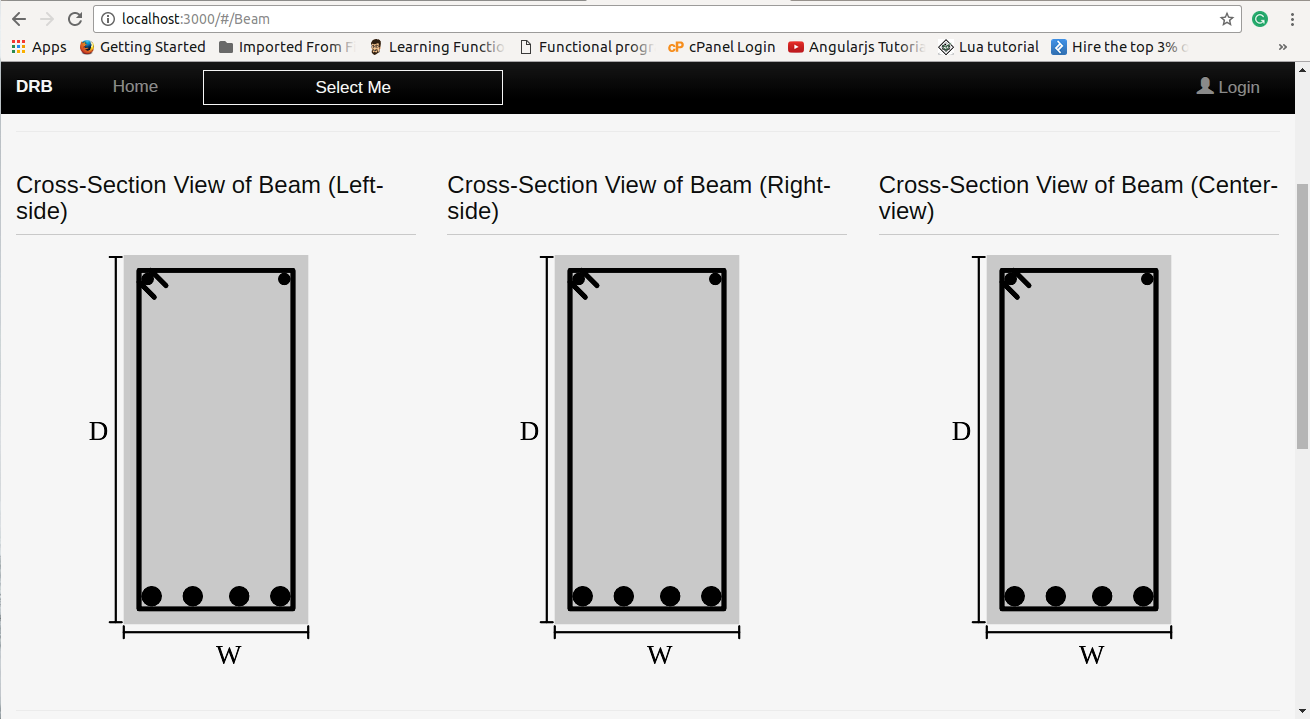
\includegraphics[scale=0.31]{images/output/screen5.png}
\caption{resulting view}
\label{fig:5}
\end{figure}

Output of the result Cross section view of beam(left, right and center)\ref{fig:4}\ref{fig:5}

\begin{figure}[H] 
\centering 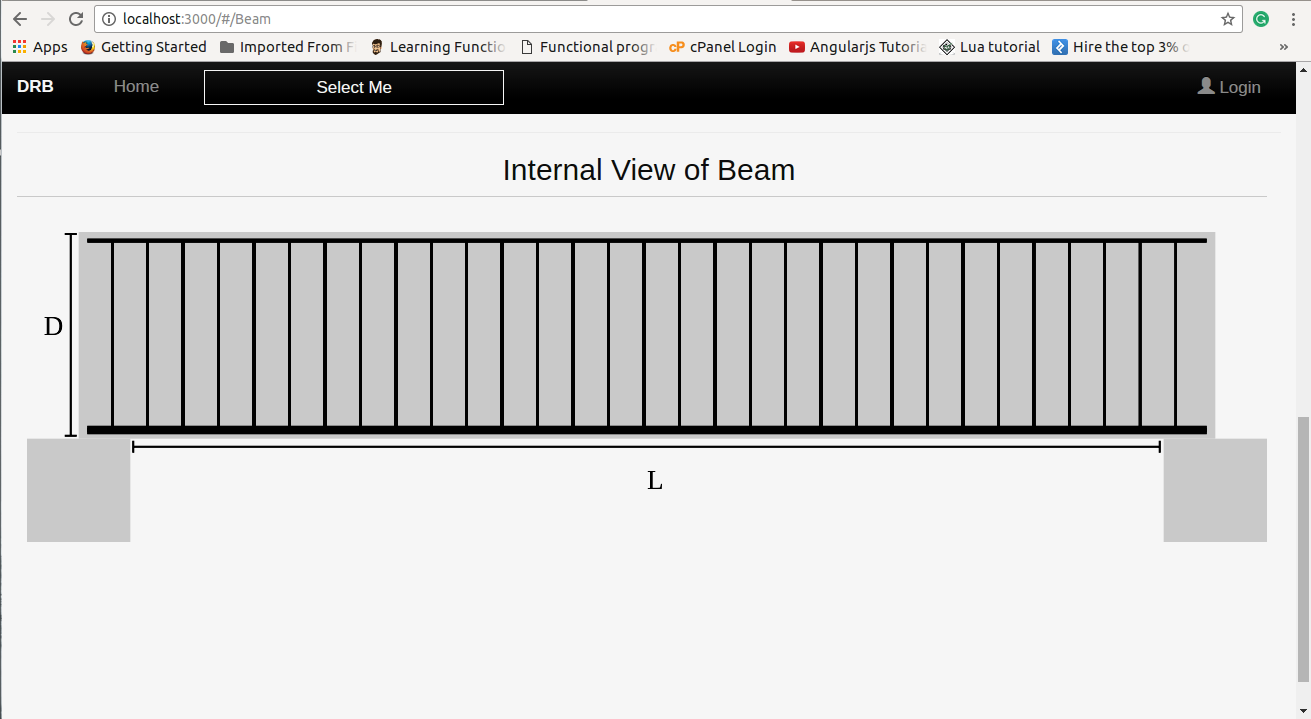
\includegraphics[scale=0.31]{images/output/screen6.png}
\caption{resulting view}
\label{fig:6}
\end{figure}

Output of the Internal view of the beam.\ref{fig:6}

\begin{figure}[H] 
\centering 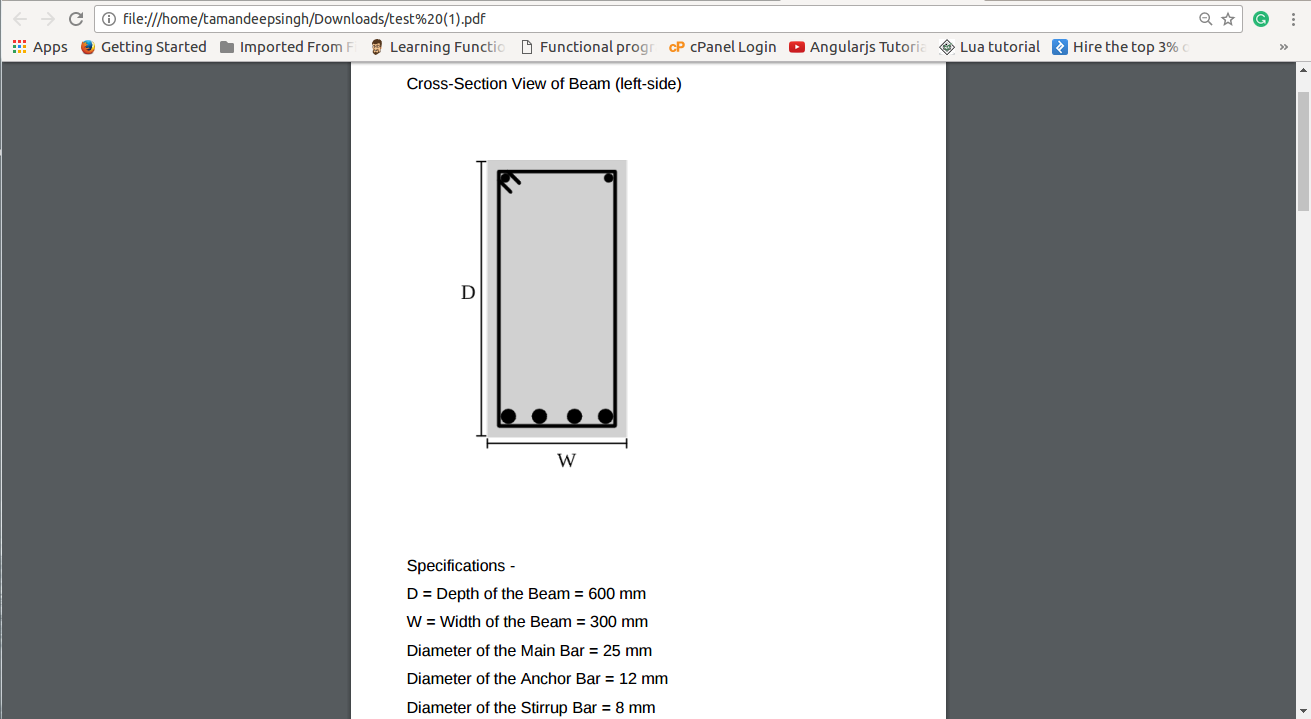
\includegraphics[scale=0.31]{images/output/screen7.png}
\caption{Result in pdf format and other information}
\label{fig:7}
\end{figure}

Output View of cross section of beam (Left side)\ref{fig:7}.

\begin{figure}[H] 
\centering 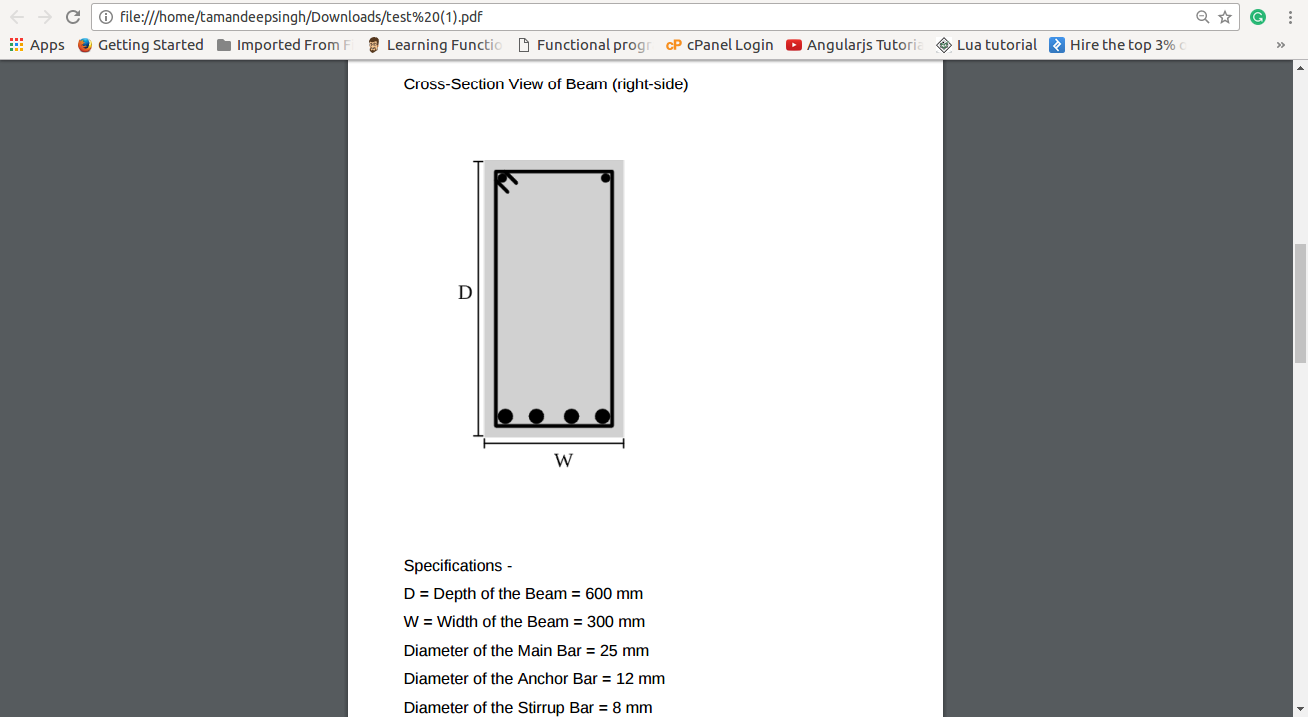
\includegraphics[scale=0.31]{images/output/screen8.png}
\caption{Result in pdf format and other information}
\label{fig:8}
\end{figure}

Output View of cross section of beam (Right side) \ref{fig:8}.

\begin{figure}[H] 
\centering 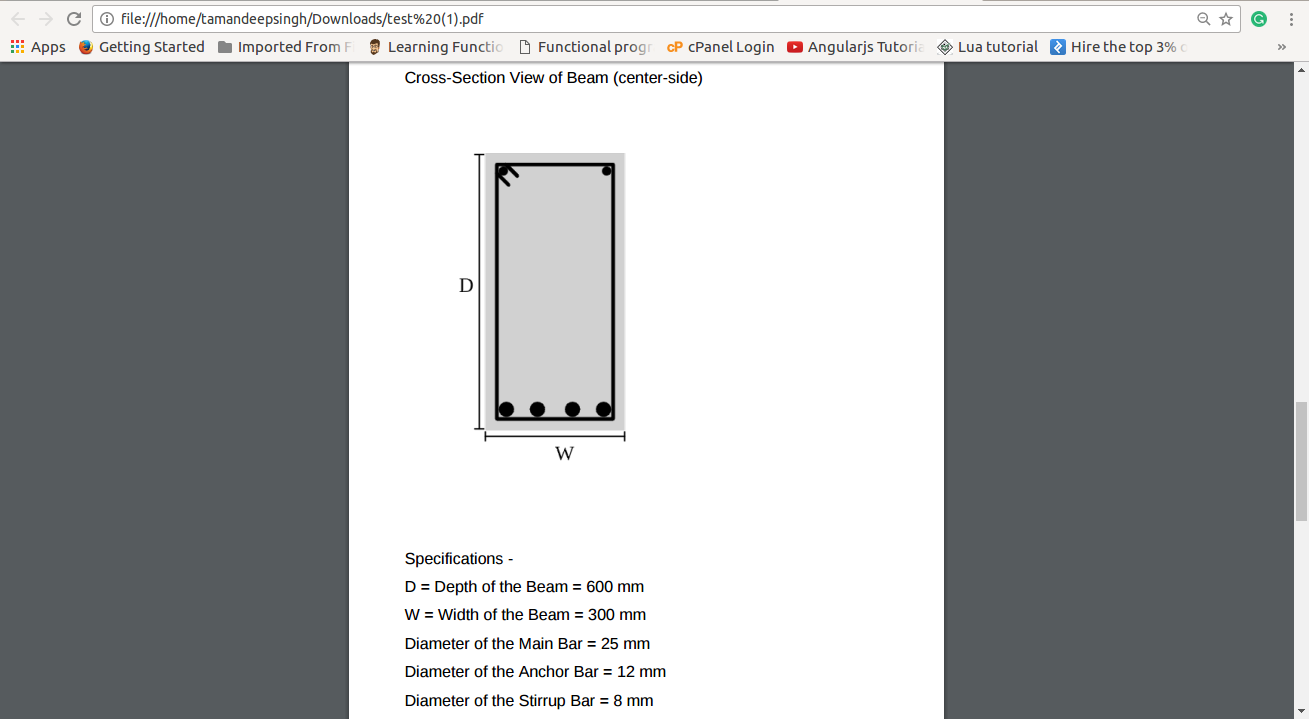
\includegraphics[scale=0.31]{images/output/screen9.png}
\caption{Result in pdf format and other information}
\label{fig:9}
\end{figure}

Output View of cross section of beam (Center side)\ref{fig:9}.

\begin{figure}[H] 
\centering 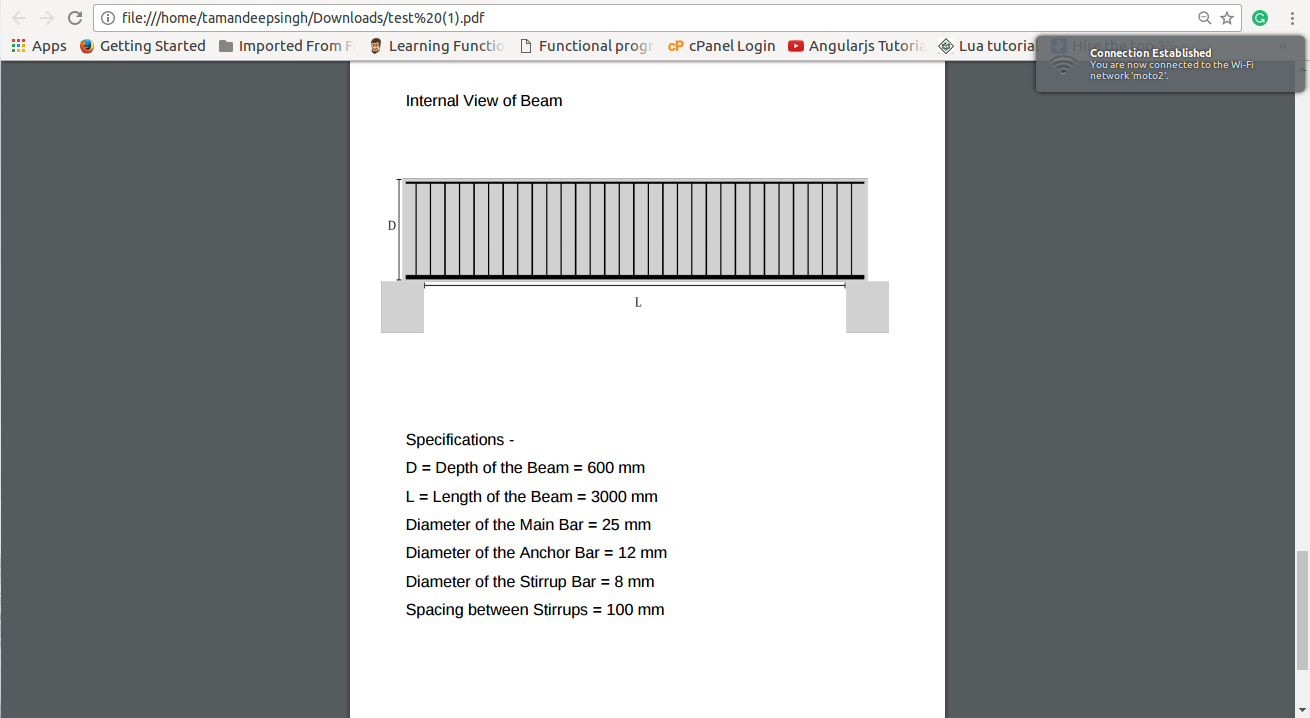
\includegraphics[scale=0.31]{images/output/screen10.png}
\caption{Result in pdf format and other information}
\label{fig:10}
\end{figure}

Output View of Internal view of the Beam\ref{fig:10}.


\chapter{CONCLUSION AND FUTURE SCOPE}
\section{Conclusion}
DRB is a very efficient application which help in generating result for analysis of structures. It
can be used by Civil Engineers and M.Tech. and B.Tech students and even layman. It's less time consuming and user-friendly 
and free from all the installation process. It is a web application that can be accessed from a number of devices. The responsive User Interface makes it easy for the users to operate it. Many efforts were made to ease the usage for the users. Hence, it is expected to be work properly in different conditions. But any future bug reports or improvements are always welcomed and will be processed happily.

I learn a lot by working on this project. During this period I got to learn a vast number of
technologies. These are listed below:
Operating system: Ubuntu
Language used: HTML, CSS and javaScript
Framework: Angular.js and Express.js
Technogloy: jspdf.js, Doxygen, Git 
So during this project I learn  all the above things. Above all I got to know how software is
developed and how much work and attention to details is required in building even the most basic
of components of any project. Planning, designing, developing code, working in a team, testing,
etc. These are all very precious lessons in themselves.
Aside from all above I got go know about various methods like -:
\begin{enumerate}
\item Threading the programs 
\item Embedding and using different tech in one software.
\item How to work like in group for development of software.
\item How to apply juggaar(innovated) in softwares to get problem solved. 
\end{enumerate}

Beside these technology used in project I also get to know some other tech also like -:
\begin{enumerate}
\item opensshserver 
\item reveal.js, impress.js (for making presentations)
\end{enumerate}  



\section{Future Scope}
This software being a open source have a lot of scope for future improvements
and additions as other individuals can also contibute in it and add additional functionality 
like-:
\begin{enumerate}
\item Output real time graph of modes 
\item Give user other anaylises option 
\item Add abiltiy to model structor online
\item Automating other anaylises techniques
\item Taking minimum amount of data and giving required result
\end{enumerate} 

\begin{thebibliography}{9}
\bibitem{} Design Reinforcement of Beam, https://github.com/TamandeepSingh/DRB
\bibitem{} \LaTeX{} https://www.sharelatex.com
\bibitem{} Node.js https://nodejs.org/en/docs/
\bibitem{} Angular.js https://docs.angularjs.org/guide/introduction
\bibitem{} My Blog, http://tamandeepsingh.wordpress.com/
\bibitem{} My Github Profile, https://github.com/TamandeepSingh
\end{thebibliography}

\end{document}

